\section{error\_\-in\_\-ly Class Reference}
\label{classerror__in__ly}\index{error_in_ly@{error\_\-in\_\-ly}}
Inheritance diagram for error\_\-in\_\-ly::\begin{figure}[H]
\begin{center}
\leavevmode
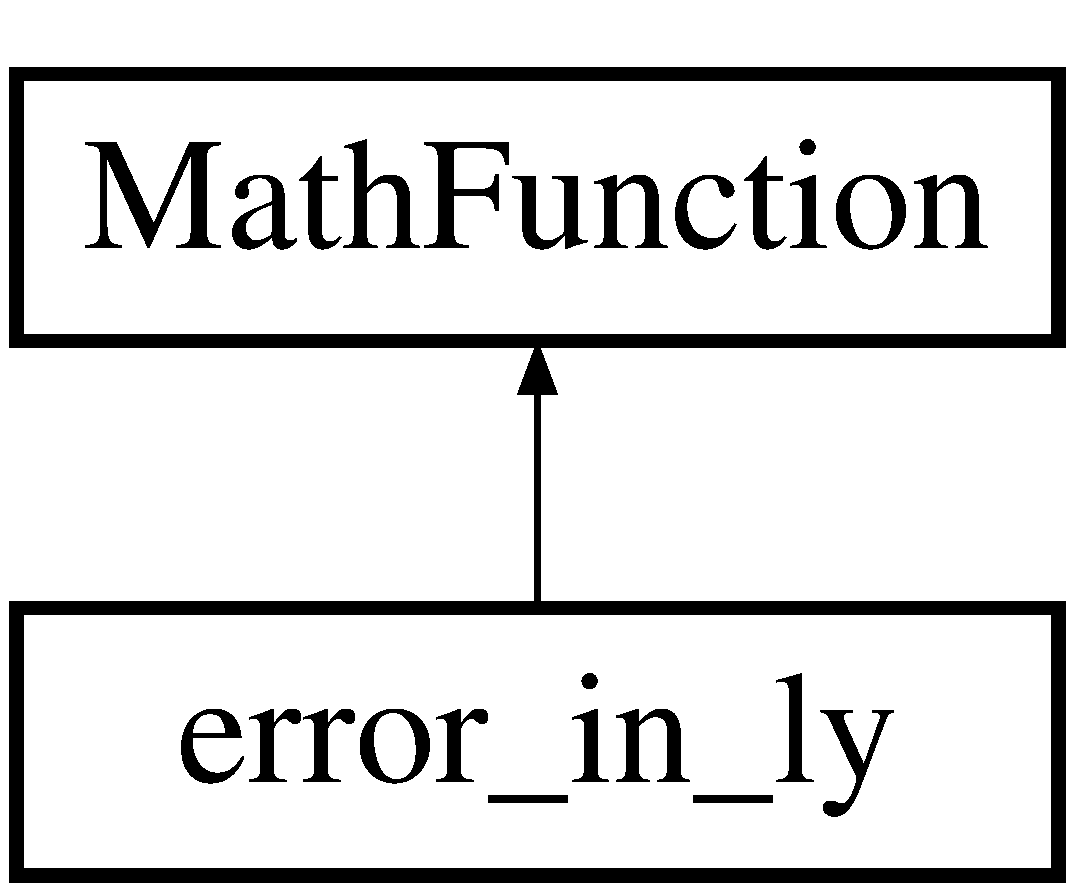
\includegraphics[height=2cm]{classerror__in__ly}
\end{center}
\end{figure}
\subsection*{Public Member Functions}
\begin{CompactItemize}
\item 
\bf{error\_\-in\_\-ly} (\bf{Double\_\-2D} const \&measured\_\-intensity, \bf{Double\_\-2D} const \&estimated\_\-intensity, double lx)\label{classerror__in__ly_b9d144e2ab980a50cf82b3cacf3db0a5}

\item 
virtual double \bf{call} (double ly)\label{classerror__in__ly_5e3f411654bc1b993a65d5a4f43f0d6d}

\end{CompactItemize}
\subsection*{Private Attributes}
\begin{CompactItemize}
\item 
double \bf{lx\_\-}\label{classerror__in__ly_b412dfc08acb49d01a49b2e5b9812b69}

\item 
\bf{Double\_\-2D} const \& \bf{estimated\_\-intensity\_\-}\label{classerror__in__ly_85bdc0e073e46d3f7497b06951747715}

\item 
\bf{Double\_\-2D} const \& \bf{measured\_\-intensity\_\-}\label{classerror__in__ly_0a61fa8b39c2c1fa63e01ab8b876d533}

\item 
std::map$<$ double, double $>$ \bf{cache}\label{classerror__in__ly_31198834676c694a170da5652c401d5d}

\end{CompactItemize}


\subsection{Detailed Description}




Definition at line 134 of file Partial\-Char\-CDI.h.

The documentation for this class was generated from the following file:\begin{CompactItemize}
\item 
Partial\-Char\-CDI.h\end{CompactItemize}
